\documentclass[border=8pt]{standalone}
\usepackage[T1]{fontenc}\usepackage{helvet}\renewcommand{\familydefault}{\sfdefault}
\usepackage{tikz}\usetikzlibrary{arrows.meta, positioning, calc, backgrounds}
\definecolor{ink}{HTML}{1a1916}
\definecolor{inktwo}{HTML}{3a3a35}
\definecolor{inkthree}{HTML}{6a6862}
\definecolor{rule}{HTML}{b8b09a}
\definecolor{amber}{HTML}{a8730a}
\definecolor{red}{HTML}{c8261a}
\definecolor{paper}{HTML}{f0eee5}
\definecolor{slab}{HTML}{d8d4c6}
\tikzset{
  >={Stealth[length=2.2mm]},
  wire/.style={line width=0.8pt, ink},
  modwire/.style={line width=0.6pt, dashed, ink},
  tastewire/.style={line width=0.6pt, dashed, amber},
  gatewire/.style={line width=0.6pt, dotted, ink},
  block/.style={rectangle, draw=ink, line width=0.9pt, fill=slab, minimum width=3.0cm, minimum height=1.9cm, inner sep=0pt},
  perf/.style={rectangle, draw=ink, line width=0.7pt, minimum width=3.0cm, minimum height=0.7cm, inner sep=2pt, font=\footnotesize, text=ink},
  title/.style={font=\scriptsize\bfseries, text=ink, anchor=north, inner sep=2pt},
  jack/.style={circle, draw=ink, fill=paper, line width=0.5pt, minimum size=3.2pt, inner sep=0pt},
  plabel/.style={font=\tiny, text=inktwo, anchor=west, inner sep=1pt},
  olabel/.style={font=\tiny, text=inktwo, anchor=east, inner sep=1pt},
  settings/.style={font=\scriptsize, text=ink, align=left, anchor=north west, inner sep=1pt, text width=2.9cm},
}
\begin{document}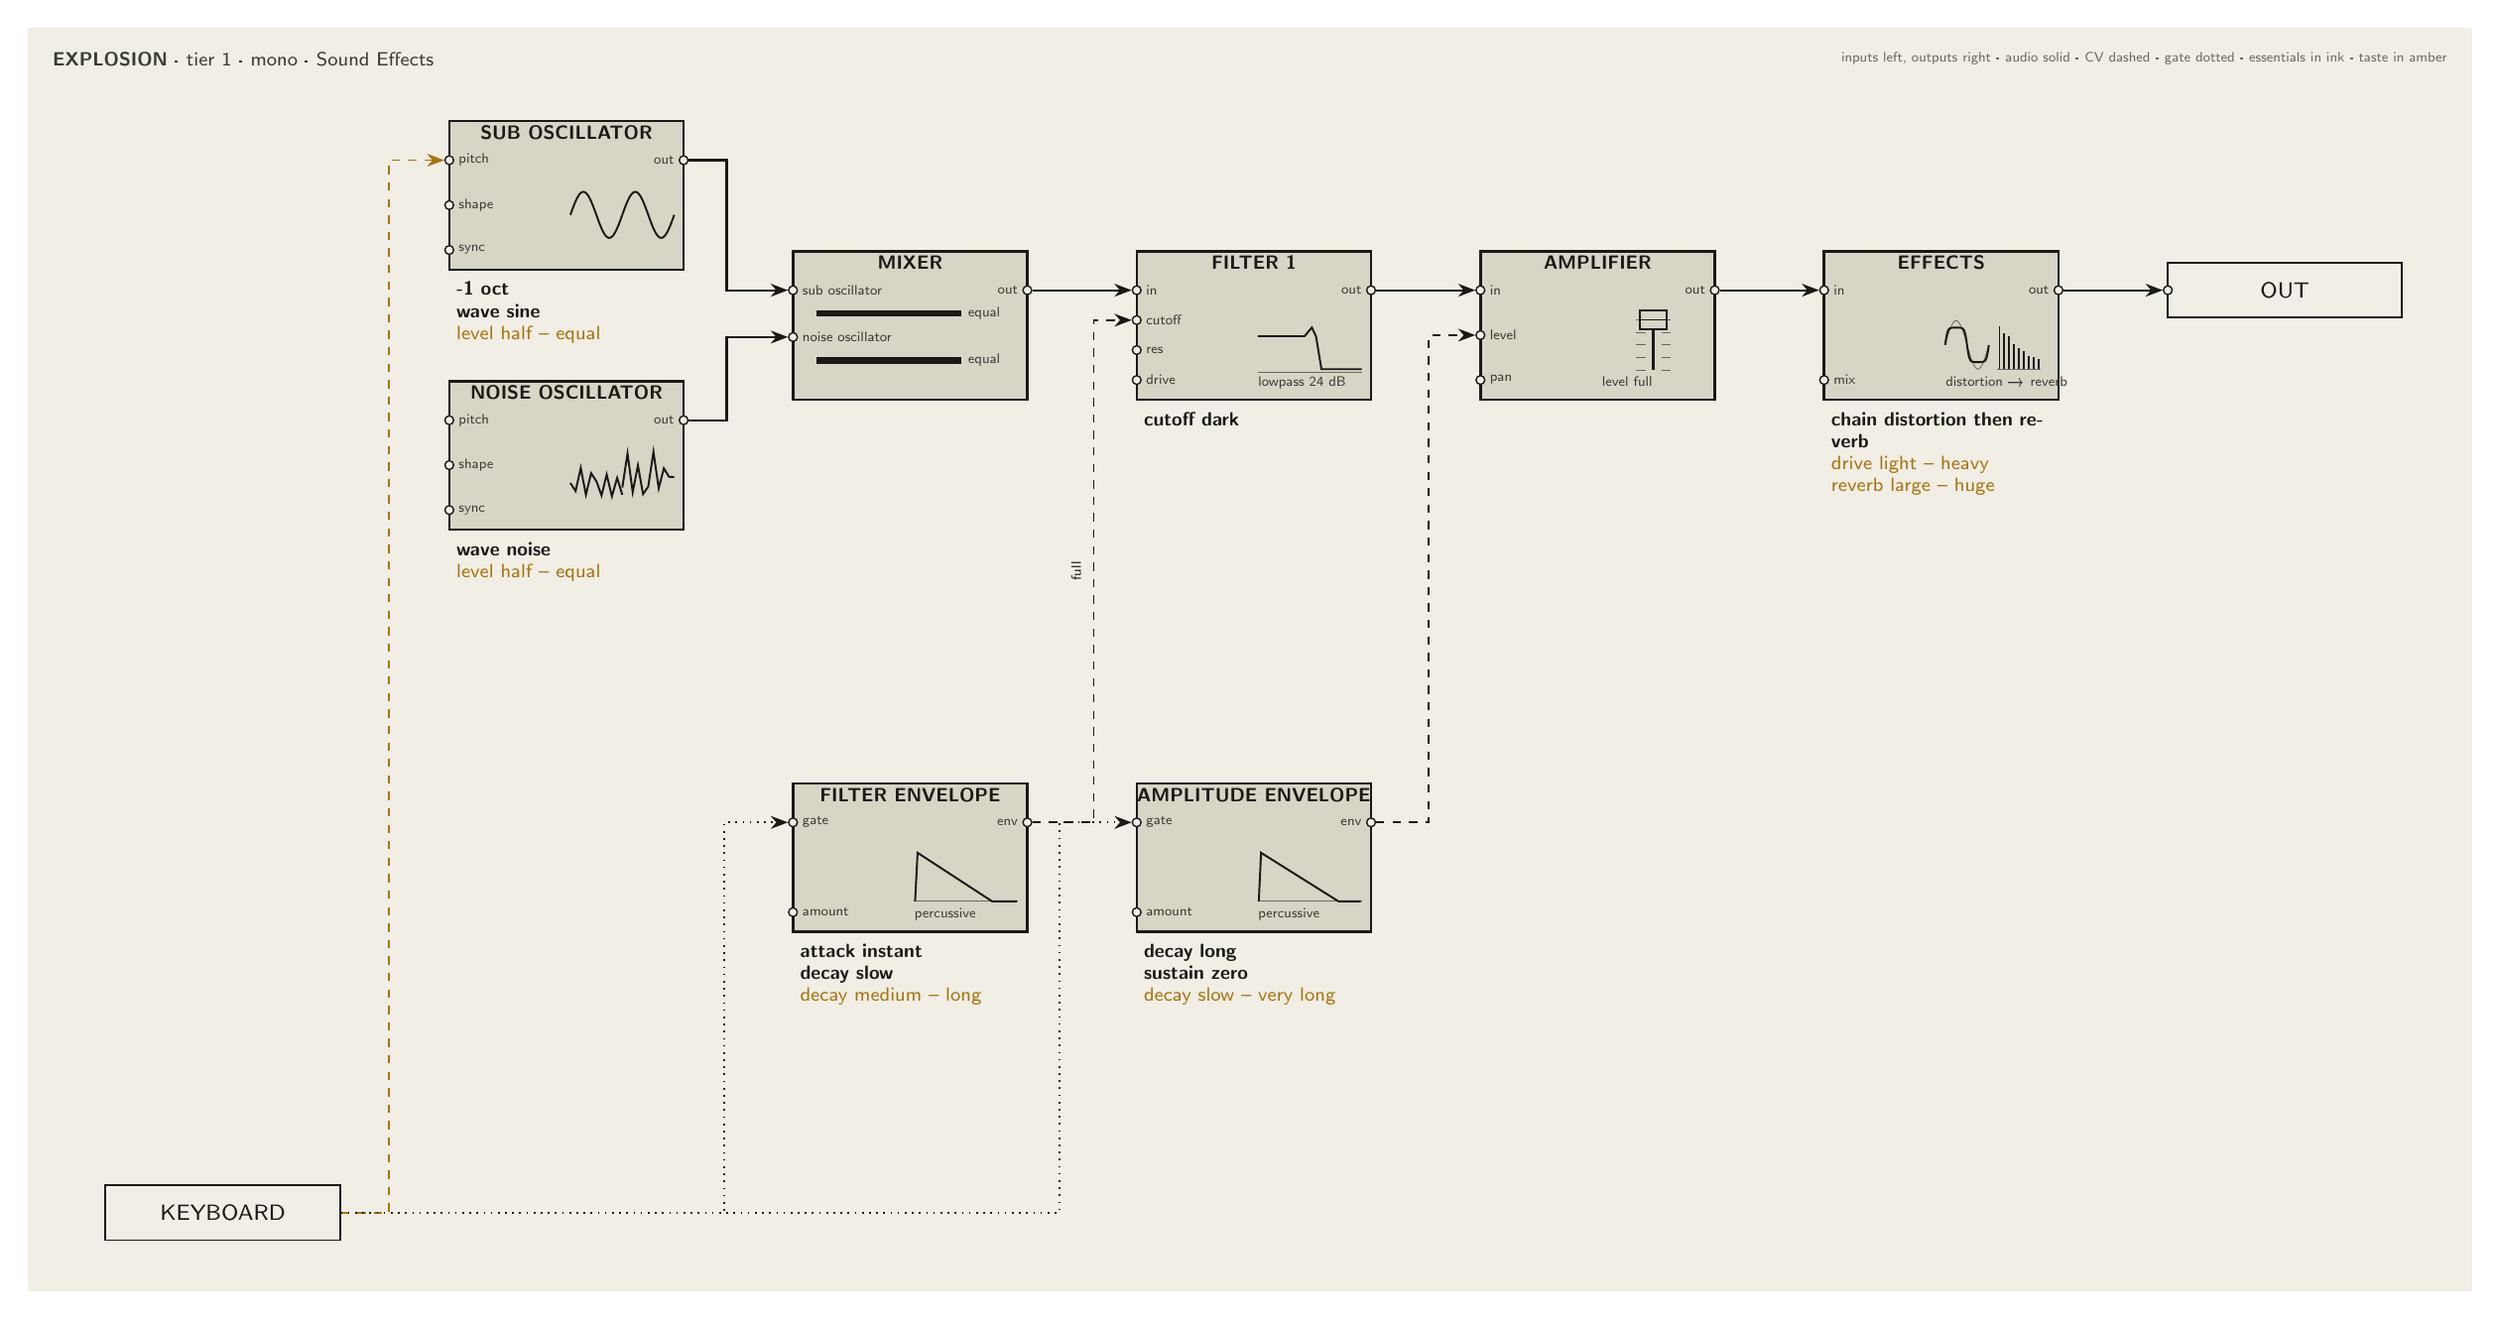
\begin{tikzpicture}
\begin{scope}[on background layer]\fill[paper] (-2.5,-12.365) rectangle (28.8,3.8150000000000004);\end{scope}
\node[block, minimum height=1.9cm] (sub) at (4.4,1.665) {};
\node[title] at (sub.north) {SUB OSCILLATOR};
\node[jack] (sub-pitch) at (2.9000000000000004,2.115) {};
\node[plabel] at (2.9800000000000004,2.115) {pitch};
\node[jack] (sub-shape) at (2.9000000000000004,1.5400000000000003) {};
\node[plabel] at (2.9800000000000004,1.5400000000000003) {shape};
\node[jack] (sub-sync) at (2.9000000000000004,0.9650000000000003) {};
\node[plabel] at (2.9800000000000004,0.9650000000000003) {sync};
\node[jack] (sub-out) at (5.9,2.115) {};
\node[olabel] at (5.82,2.115) {out};
\begin{scope}
\draw[ink, line width=0.7pt] plot[domain=0.000:0.500, samples=24, variable=\u] ({4.450+\u*1.330},{1.045+(0.740)*(0.5+0.4*sin(360*(\u*2))+0.0)});
\draw[ink, line width=0.7pt] plot[domain=0.500:1.000, samples=24, variable=\u] ({4.450+\u*1.330},{1.045+(0.740)*(0.5+0.4*sin(360*(\u*2))+0.0)});
\end{scope}
\node[settings] at (2.95,0.5950000000000001) {\textbf{-1 oct} \\ \textbf{wave sine} \\ \textcolor{amber}{level half -- equal}};
\node[block, minimum height=1.9cm] (noise) at (4.4,-1.665) {};
\node[title] at (noise.north) {NOISE OSCILLATOR};
\node[jack] (noise-pitch) at (2.9000000000000004,-1.215) {};
\node[plabel] at (2.9800000000000004,-1.215) {pitch};
\node[jack] (noise-shape) at (2.9000000000000004,-1.79) {};
\node[plabel] at (2.9800000000000004,-1.79) {shape};
\node[jack] (noise-sync) at (2.9000000000000004,-2.365) {};
\node[plabel] at (2.9800000000000004,-2.365) {sync};
\node[jack] (noise-out) at (5.9,-1.215) {};
\node[olabel] at (5.82,-1.215) {out};
\begin{scope}
\draw[ink, line width=0.7pt] (4.450,-2.019) -- (4.517,-2.122) -- (4.583,-1.826) -- (4.649,-2.168) -- (4.716,-1.894) -- (4.783,-1.995) -- (4.849,-2.177) -- (4.915,-1.911) -- (4.982,-2.189) -- (5.049,-1.954) -- (5.115,-2.170);
\draw[ink, line width=0.7pt] (5.115,-2.077) -- (5.182,-1.641) -- (5.248,-2.136) -- (5.315,-1.794) -- (5.381,-2.161) -- (5.447,-2.065) -- (5.514,-1.620) -- (5.581,-2.087) -- (5.647,-1.831) -- (5.713,-1.939) -- (5.780,-1.943);
\end{scope}
\node[settings] at (2.95,-2.7350000000000003) {\textbf{wave noise} \\ \textcolor{amber}{level half -- equal}};
\node[block, minimum height=1.9cm] (mix) at (8.8,0.0) {};
\node[title] at (mix.north) {MIXER};
\node[jack] (mix-sub) at (7.300000000000001,0.44999999999999996) {};
\node[plabel] at (7.380000000000001,0.44999999999999996) {sub oscillator};
\draw[inkthree, line width=0.3pt] (7.600,0.150) -- (9.450,0.150);
\draw[ink, line width=2.2pt] (7.600,0.150) -- (9.450,0.150);
\node[font=\tiny, text=inktwo, anchor=west, inner sep=1pt] at (9.500,0.150) {equal};
\node[jack] (mix-noise) at (7.300000000000001,-0.15000000000000002) {};
\node[plabel] at (7.380000000000001,-0.15000000000000002) {noise oscillator};
\draw[inkthree, line width=0.3pt] (7.600,-0.450) -- (9.450,-0.450);
\draw[ink, line width=2.2pt] (7.600,-0.450) -- (9.450,-0.450);
\node[font=\tiny, text=inktwo, anchor=west, inner sep=1pt] at (9.500,-0.450) {equal};
\node[jack] (mix-out) at (10.3,0.44999999999999996) {};
\node[olabel] at (10.22,0.44999999999999996) {out};
\node[block, minimum height=1.9cm] (filter1) at (13.200000000000001,0.0) {};
\node[title] at (filter1.north) {FILTER 1};
\node[jack] (filter1-in) at (11.700000000000001,0.44999999999999996) {};
\node[plabel] at (11.780000000000001,0.44999999999999996) {in};
\node[jack] (filter1-cutoff) at (11.700000000000001,0.06666666666666665) {};
\node[plabel] at (11.780000000000001,0.06666666666666665) {cutoff};
\node[jack] (filter1-res) at (11.700000000000001,-0.31666666666666665) {};
\node[plabel] at (11.780000000000001,-0.31666666666666665) {res};
\node[jack] (filter1-drive) at (11.700000000000001,-0.7) {};
\node[plabel] at (11.780000000000001,-0.7) {drive};
\node[jack] (filter1-out) at (14.700000000000001,0.44999999999999996) {};
\node[olabel] at (14.620000000000001,0.44999999999999996) {out};
\begin{scope}
\draw[inkthree, line width=0.3pt] (13.250,-0.605) -- (14.580,-0.605);
\draw[ink, line width=0.7pt] (13.250,-0.139) -- (13.849,-0.139) -- (13.942,-0.028) -- (13.995,-0.139) -- (14.065,-0.561) -- (14.580,-0.561);
\node[font=\tiny, text=inktwo, anchor=north west, inner sep=0pt] at (13.250,-0.650) {lowpass 24 dB};
\end{scope}
\node[settings] at (11.750000000000002,-1.0699999999999998) {\textbf{cutoff dark}};
\node[block, minimum height=1.9cm] (amp) at (17.6,0.0) {};
\node[title] at (amp.north) {AMPLIFIER};
\node[jack] (amp-in) at (16.1,0.44999999999999996) {};
\node[plabel] at (16.18,0.44999999999999996) {in};
\node[jack] (amp-level) at (16.1,-0.125) {};
\node[plabel] at (16.18,-0.125) {level};
\node[jack] (amp-pan) at (16.1,-0.7) {};
\node[plabel] at (16.18,-0.7) {pan};
\node[jack] (amp-out) at (19.1,0.44999999999999996) {};
\node[olabel] at (19.020000000000003,0.44999999999999996) {out};
\begin{scope}
\draw[ink, line width=1.2pt] (18.315,-0.570) -- (18.315,0.070);
\draw[inkthree, line width=0.3pt] (18.095,-0.570) -- (18.215,-0.570) (18.415,-0.570) -- (18.535,-0.570);
\draw[inkthree, line width=0.3pt] (18.095,-0.410) -- (18.215,-0.410) (18.415,-0.410) -- (18.535,-0.410);
\draw[inkthree, line width=0.3pt] (18.095,-0.250) -- (18.215,-0.250) (18.415,-0.250) -- (18.535,-0.250);
\draw[inkthree, line width=0.3pt] (18.095,-0.090) -- (18.215,-0.090) (18.415,-0.090) -- (18.535,-0.090);
\draw[inkthree, line width=0.3pt] (18.095,0.070) -- (18.215,0.070) (18.415,0.070) -- (18.535,0.070);
\fill[slab, draw=ink, line width=0.6pt] (18.145,-0.050) rectangle (18.485,0.190);
\draw[ink, line width=0.5pt] (18.145,0.070) -- (18.485,0.070);
\node[font=\tiny, text=inktwo, anchor=north west, inner sep=0pt] at (17.650,-0.650) {level full};
\end{scope}
\node[block, minimum height=1.9cm] (fx) at (22.0,0.0) {};
\node[title] at (fx.north) {EFFECTS};
\node[jack] (fx-in) at (20.5,0.44999999999999996) {};
\node[plabel] at (20.58,0.44999999999999996) {in};
\node[jack] (fx-mix) at (20.5,-0.7) {};
\node[plabel] at (20.58,-0.7) {mix};
\node[jack] (fx-out) at (23.5,0.44999999999999996) {};
\node[olabel] at (23.42,0.44999999999999996) {out};
\begin{scope}
\draw[inkthree, line width=0.3pt] plot[domain=0.000:0.420, samples=30, variable=\u] ({22.050+\u*1.330},{-0.620+(0.740)*(0.5+0.42*sin(360*((\u-0.000)/0.420)))});
\draw[ink, line width=0.7pt] plot[domain=0.000:0.420, samples=40, variable=\u] ({22.050+\u*1.330},{-0.620+(0.740)*(0.5+0.3*tanh(3*sin(360*((\u-0.000)/0.420))))});
\draw[inkthree, line width=0.3pt] (22.715,-0.561) -- (23.274,-0.561);
\draw[ink, line width=0.6pt] (22.743,-0.561) -- (22.743,-0.018);
\draw[ink, line width=0.6pt] (22.806,-0.561) -- (22.806,-0.095);
\draw[ink, line width=0.6pt] (22.869,-0.561) -- (22.869,-0.133);
\draw[ink, line width=0.6pt] (22.931,-0.561) -- (22.931,-0.246);
\draw[ink, line width=0.6pt] (22.994,-0.561) -- (22.994,-0.296);
\draw[ink, line width=0.6pt] (23.057,-0.561) -- (23.057,-0.335);
\draw[ink, line width=0.6pt] (23.120,-0.561) -- (23.120,-0.394);
\draw[ink, line width=0.6pt] (23.183,-0.561) -- (23.183,-0.408);
\draw[ink, line width=0.6pt] (23.246,-0.561) -- (23.246,-0.429);
\node[font=\tiny, text=inktwo, anchor=north west, inner sep=0pt] at (22.050,-0.650) {distortion → reverb};
\end{scope}
\node[settings] at (20.55,-1.0699999999999998) {\textbf{chain distortion then reverb} \\ \textcolor{amber}{drive light -- heavy} \\ \textcolor{amber}{reverb large -- huge}};
\node[block, minimum height=1.9cm] (fenv) at (8.8,-6.815) {};
\node[title] at (fenv.north) {FILTER ENVELOPE};
\node[jack] (fenv-gate) at (7.300000000000001,-6.365) {};
\node[plabel] at (7.380000000000001,-6.365) {gate};
\node[jack] (fenv-amount) at (7.300000000000001,-7.515000000000001) {};
\node[plabel] at (7.380000000000001,-7.515000000000001) {amount};
\node[jack] (fenv-out) at (10.3,-6.365) {};
\node[olabel] at (10.22,-6.365) {env};
\begin{scope}
\draw[inkthree, line width=0.3pt] (8.850,-7.376) -- (10.180,-7.376);
\draw[ink, line width=0.7pt] (8.863,-7.376) -- (8.895,-6.754) -- (9.849,-7.376) -- (9.849,-7.376) -- (10.167,-7.376);
\node[font=\tiny, text=inktwo, anchor=north west, inner sep=0pt] at (8.850,-7.465) {percussive};
\end{scope}
\node[settings] at (7.3500000000000005,-7.885000000000001) {\textbf{attack instant} \\ \textbf{decay slow} \\ \textcolor{amber}{decay medium -- long}};
\node[block, minimum height=1.9cm] (aenv) at (13.200000000000001,-6.815) {};
\node[title] at (aenv.north) {AMPLITUDE ENVELOPE};
\node[jack] (aenv-gate) at (11.700000000000001,-6.365) {};
\node[plabel] at (11.780000000000001,-6.365) {gate};
\node[jack] (aenv-amount) at (11.700000000000001,-7.515000000000001) {};
\node[plabel] at (11.780000000000001,-7.515000000000001) {amount};
\node[jack] (aenv-out) at (14.700000000000001,-6.365) {};
\node[olabel] at (14.620000000000001,-6.365) {env};
\begin{scope}
\draw[inkthree, line width=0.3pt] (13.250,-7.376) -- (14.580,-7.376);
\draw[ink, line width=0.7pt] (13.263,-7.376) -- (13.292,-6.754) -- (14.283,-7.376) -- (14.283,-7.376) -- (14.567,-7.376);
\node[font=\tiny, text=inktwo, anchor=north west, inner sep=0pt] at (13.250,-7.465) {percussive};
\end{scope}
\node[settings] at (11.750000000000002,-7.885000000000001) {\textbf{decay long} \\ \textbf{sustain zero} \\ \textcolor{amber}{decay slow -- very long}};
\node[perf] (key) at (0.0,-11.365) {KEYBOARD};
\node[perf, fill=paper] (out) at (26.400000000000002,0.44999999999999996) {OUT}; \node[jack] (out-in) at (24.900000000000002,0.44999999999999996) {};
\draw[wire,->] (sub-out) -- (6.45,2.115) |- (mix-sub);
\draw[wire,->] (noise-out) -- (6.45,-1.215) |- (mix-noise);
\draw[wire,->] (mix-out) -- (filter1-in);
\draw[wire,->] (filter1-out) -- (amp-in);
\draw[wire,->] (amp-out) -- (fx-in);
\draw[wire,->] (fx-out) -- (out-in);
\draw[modwire,->] (fenv-out) -- (11.15,-6.365) -- (11.15,0.06666666666666665) -- (filter1-cutoff);
\node[font=\tiny, text=ink, anchor=south, inner sep=1pt, rotate=90] at (11.030000000000001,-3.149166666666667) {full};
\draw[modwire,->] (aenv-out) -- (15.440000000000001,-6.365) -- (15.440000000000001,-0.125) -- (amp-level);
\draw[tastewire,->] (key.east) -- (2.1300000000000003,-11.365) -- (2.1300000000000003,2.115) -- (sub-pitch);
\draw[gatewire,->] (key.east) -- (6.420000000000001,-11.365) -- (6.420000000000001,-6.365) -- (fenv-gate);
\draw[gatewire,->] (key.east) -- (10.71,-11.365) -- (10.71,-6.365) -- (aenv-gate);
\node[anchor=north west, font=\scriptsize, text=inktwo] at (-2.3,3.615) {\textbf{EXPLOSION} · tier 1 · mono · Sound Effects};
\node[anchor=north east, font=\tiny, text=inkthree] at (28.6,3.615) {inputs left, outputs right · audio solid · CV dashed · gate dotted · essentials in ink · taste in amber};
\end{tikzpicture}\end{document}
